% The \vspace{} command in this chapter is just for aesthetic reasons - I don't like something new to start at the last line 
%of the page

% ONE OF THE BEST ONLINE LATEX REFERENCES IS AT :
% http://www.eng.cam.ac.uk/help/tpl/textprocessing/latex_advanced/latex_advanced.html

%% ALL figures are in EPS format: It is the best possible format 

%Some ideas:

%\begin{itemize}
%
%\item The Zebrafish Mincle
%\item Sufficiency
%\item Cotranscriptional interplay
%\item Integration of HIF-1$\upalpha$ signaling
%\item Lymphangiogenesis
%\item Aspects that differentiate the isoforms in macrophages
%\item Effect of NFAT mutation on macrophage biology
%\item Mycobacterial interactions with other vasculature-relevant features -- plasmin, TIE2, fibronectin, etc.
%\item Role of NFAT in neutrophils
%\item New tools to study this pathway \textit{in vivo}
%\item Generalizability
%\item Novel Methods to Automate Measurement of Angiogenesis
%\item Novel Methods to Automate Cell Feature Quantitation
%\item Other Contributions of NFAT to Host-Mycobacterial Interactions
%\item Promise as a Host-Directed Therapy
%
%\end{itemize}

At the conclusion of the present work, many new questions have been generated while others remain unanswered. This work has accomplished two primary goals: addressing the intracellular signaling pathway within macrophages that is responsible for inducing angiogenesis during mycobacterial infection (the NFAT pathway) and setting the stage for future work to simplify and automate common procedures commonly used in the analysis of imaging data relevant to both zebrafish and tissue culture research. Some of these lingering questions will be addressed in the coming weeks and months while others will stretch over the course of many years or decades as we delve into deeper and deeper understandings of the fundamental processes governing the nature of the angiogenic response to tuberculosis infection and how and when this can be a fruitful target for therapeutic intervention. 

This leaves a set of important questions, pertinent to model development, deeper understanding of the biology of NFAT within (granuloma) macrophages, the intersections between this pathway and other, known pathways involved in angiogenic responses, and the future of imaging analysis in the context of ever-growing computational power. 

\begin{itemize}
\item What is the TDM receptor in zebrafish and do they have an as-yet unannotated MINCLE homolog? 
\item How or why is NFATC2 special and is it sufficient to induce VEGF? 
\item How does the NFAT pathway alter other aspects of macrophage behavior potentially relevant to tuberculosis biology and does this pathway intersect with HIF-1$\upalpha$ signaling? 
\item Aside from TDM, do mycobacteria have other mechanisms for manipulating the host angiogenic response and, if so, what are they and how does that enhance our overall understanding of this process? 
\item Are our findings on the nature of NFATC2 in inducing tuberculous angiogenesis relevant to other disease contexts where VEGF signaling plays an important role? 
\item Could NFAT offer a meaningful mechanism for inhibiting angiogenesis in the context of disease as a host-directed therapy?
\end{itemize}

These questions, among many others, are the subject of this concluding chapter; it is hoped that a comprehensive presentation of these questions will stimulate future generations to pursue answers and that these will further inform our understanding of the pathogenesis of tuberculosis toward the goal of eradicating this disease.

\section{The Zebrafish MINCLE}

As discussed in \autoref{tdmreceptor}, data from human cell culture and mice has implicated MCL and MINCLE as the primary C-type lectin receptors for TDM, which induces a variety of downstream responses, seemingly including the upregulation of VEGF and downstream angiogenesis (see \autoref{chap3}). However, the precise identity of the homolog of MCL or MINCLE in the zebrafish remains unknown. These two proteins arose from a tandem duplication and inversion at an unknown point in evolutionary history, although the two are ubiquitous across reptiles, birds, and mammals \citep{Miyake2013, Richardson2014}. Given the strong, bidirectional selective pressure on both host and pathogen to modulate host PRR activity, these divergences are expected even between closely related species \citep{Rambaruth2015}. This diversification is especially notable among CLRs: mice have no fewer than eight putative DC-SIGN homologs and a great deal of work was done to narrow down the functional ones in order to model human disease \citep{GarciaVallejo2013}; on the other hand, the bovine homolog of MINCLE was readily identifiable but had diverged in non-critical domains from the human MINCLE \citep{Feinberg2016, Furukawa2013, Feinberg2013}. Indeed, the murine Mincle is only 67\% identical to the human MINCLE, despite an overlapping set of known ligands \citep{Matsumoto1999}. These aspects of structural diversity add unique complexities to the identification of any putative functional homolog in the fish, which may have substantially diverged from the ancestral protein as well as the mammalian versions. Despite these challenges, such identification would both substantially advance the zebrafish\hyp{}\textit{M. marinum} model and deepen our understanding of shared mechanisms of detection and response to C-type lectin receptor ligands.

Despite these challenges, there is an abundance of evidence that zebrafish possess an as-yet unidentified MINCLE (and/or MCL) homolog including, but not limited to: a long evolutionary history alongside pathogenic mycobacteria, the clear, \textit{myd88}-independent inflammatory response to purified TDM, and the \textit{in vivo} attenuation of mutants lacking fully mature TDM. Zebrafish have long been speculated to have functional homologs of other C-type lectin receptors despite difficulty in their identification \citep{Petit2019}. MINCLE has not been previously linked to angiogenesis, but the identification of this receptor in zebrafish would allow us to better understand the relevant pathway in humans; indeed, the role of MINCLE during infection is unclear given that some groups have demonstrated that it contributes to bacterial control while others have seen no effect \citep{Behler2012, Behler2015, Heitmann2013, Lee2012}. This has translational implications for modulating the activity of the human MINCLE to enrich for host-beneficial responses and also basic science implications in revealing the diversification of a receptor that maintains the ability to detect a common ligand. 

Unlike MINCLE, the basal receptor MCL has clear roles in mediating protection against mycobacteria \citep{Wilson2015}. This might imply that the basal recognition capacities of MCL and potentially later downstream events that depend on MCL/MINCLE interactions are more important than the contributions of MINCLE alone. What is needed is a full locus-deletion mouse that removes both MCL and MINCLE to enable studies on the function of TDM detection \textit{per se} \textit{in vivo}. While the development of a mouse model to accomplish this would be an excellent contribution, we may be able to fill in some gaps using the zebrafish if we are able to identify the correct homolog in the zebrafish genome.

Although large amino acid segments of CLRs are able to undergo radical changes in primary sequence with few deleterious effects, there are several domains that have been identified as absolutely essential for binding to TDM. A specific set of criteria for this selection are listed in \autoref{minctab} \citep{Alenton2017, Feinberg2016, Feinberg2013, Bird2018, Furukawa2013, Zelensky2005}. Based on these criteria, we have identified three putative homologs with $>$50\% amino acid similarity to the human CLEC4E in the carbohydrate binding domain (\autoref{minctab}) and have identified transmitting nonsense mutations in each of them (\autoref{zfmincs}). As further evidence, two of these homologs (77975 and 79903) are organized in tandem, mirroring the genomic organization of MINCLE and MCL in mammals. 

\singlespacing
\begin{center}
\begin{longtable}{|>{\raggedright\arraybackslash}m{1.5in}|>{\raggedright\arraybackslash}m{4in}|}
\caption{Criteria used to select putative zebrafish homologs of the human MINCLE.}\label{minctab} \tabularnewline

\hline
\thead{Criteria} & \thead{Rationale} \tabularnewline
\hline
Possesses a gEPNn motif & Of the two major carbohydrate recognition domain motifs, the EPN motif is known to bind glucose-derived sugars while QPD motifs are known to bind galactose-derived sugars. As trehalose is a di-glucose and MINCLE and MCL both possess this EPN motif, this is an important first-pass selection criterion. \tabularnewline
\hline
Lacks an intracellular ITAM motif & In humans, both MINCLE and MCL use Fc$\upgamma$R to signal as they lack their own ITAM motif. While not an essential quality to detect and respond to TDM, this would strengthen the similarities between the two; we have also published data implicating Fc$\upgamma$R in the zebrafish, which argues in favor of this shared layer of similarity as well. \tabularnewline
\hline
Induced by infection & Using existing RNA-seq datasets, expression of these genes under inflammatory stimulus is an important indicator that they may be acting similarly to MINCLE, which is an inducible gene responsive to various inflammatory stimuli. \tabularnewline
\hline
Transmembrane helix & These surface receptors use a single-pass transmembrane helix to remain bound to the plasma membrane and transduce signals. \tabularnewline
\hline
Hydrophobic amino acids in the CRD & One of the defining biochemical features of MINCLE is a small hydrophobic pocket that appears to be useful for binding to the mycolate tails of TDM; the presence of such a pocket would be evocative of further similarity to MINCLE. \tabularnewline
\hline

\end{longtable}
\end{center}

\doublespacing

Multiple approaches can be taken to identify the capacity of these proteins to bind TDM and generate meaningful biological responses. Going forward, I propose to take a biochemistry-first approach to this question as it enables greater flexibility in responding to new data and starts with a foundation of known interactions. Thus, I will utilize established methods of TDM blotting \citep{Jegouzo2014} and wash recombinant carbohydrate recognition domain-streptavidin fusion protein lysate across them and then detect these interactions using standard biotin-horseradish peroxidase detection. This will provide a quantifiable readout for both presence/absence of an interaction but also the strength of the interaction. Should none of these proteins efficiently bind TDM, it is relatively trivial to generate new chimeric proteins and test a range of others present in the zebrafish genome. This data can then be used to go back into the zebrafish to assess the \textit{in vivo} consequences of this interaction and also allow for more flexibility in approach -- rather that seeking the receptor, we can explore phenotypes that may be altered in this context across both angiogenic responses and more general immune responses.

In the zebrafish itself, I would actually propose to take a few steps backward and return to a mosaic-based screening approach. While the long-term goal should be to generate a full locus-spanning deletion of 77975 and 79903, it may be worthwhile to use the zebrafish as a screening platform to determine the potential contributions of these two genes separately and together in the angiogenesis phenotype and CRISPR/Cas9 ribonucleoprotein injections allow for such rapid screening and planning for whether it makes sense to invest the time and energy in generating a full deletion mutant. Given the unlikelihood of being able to ever generate a crossover event to combine the two existing mutations, some alternative approach is clearly going to be required and this seems like a great place to start in pursuit of the zebrafish MCL/MINCLE. These two genes make for especially compelling candidates as they are macrophage-specific and are induced by infection, even in bystander macrophages \autoref{figure:mincles}. 

\begin{figure}
\centering
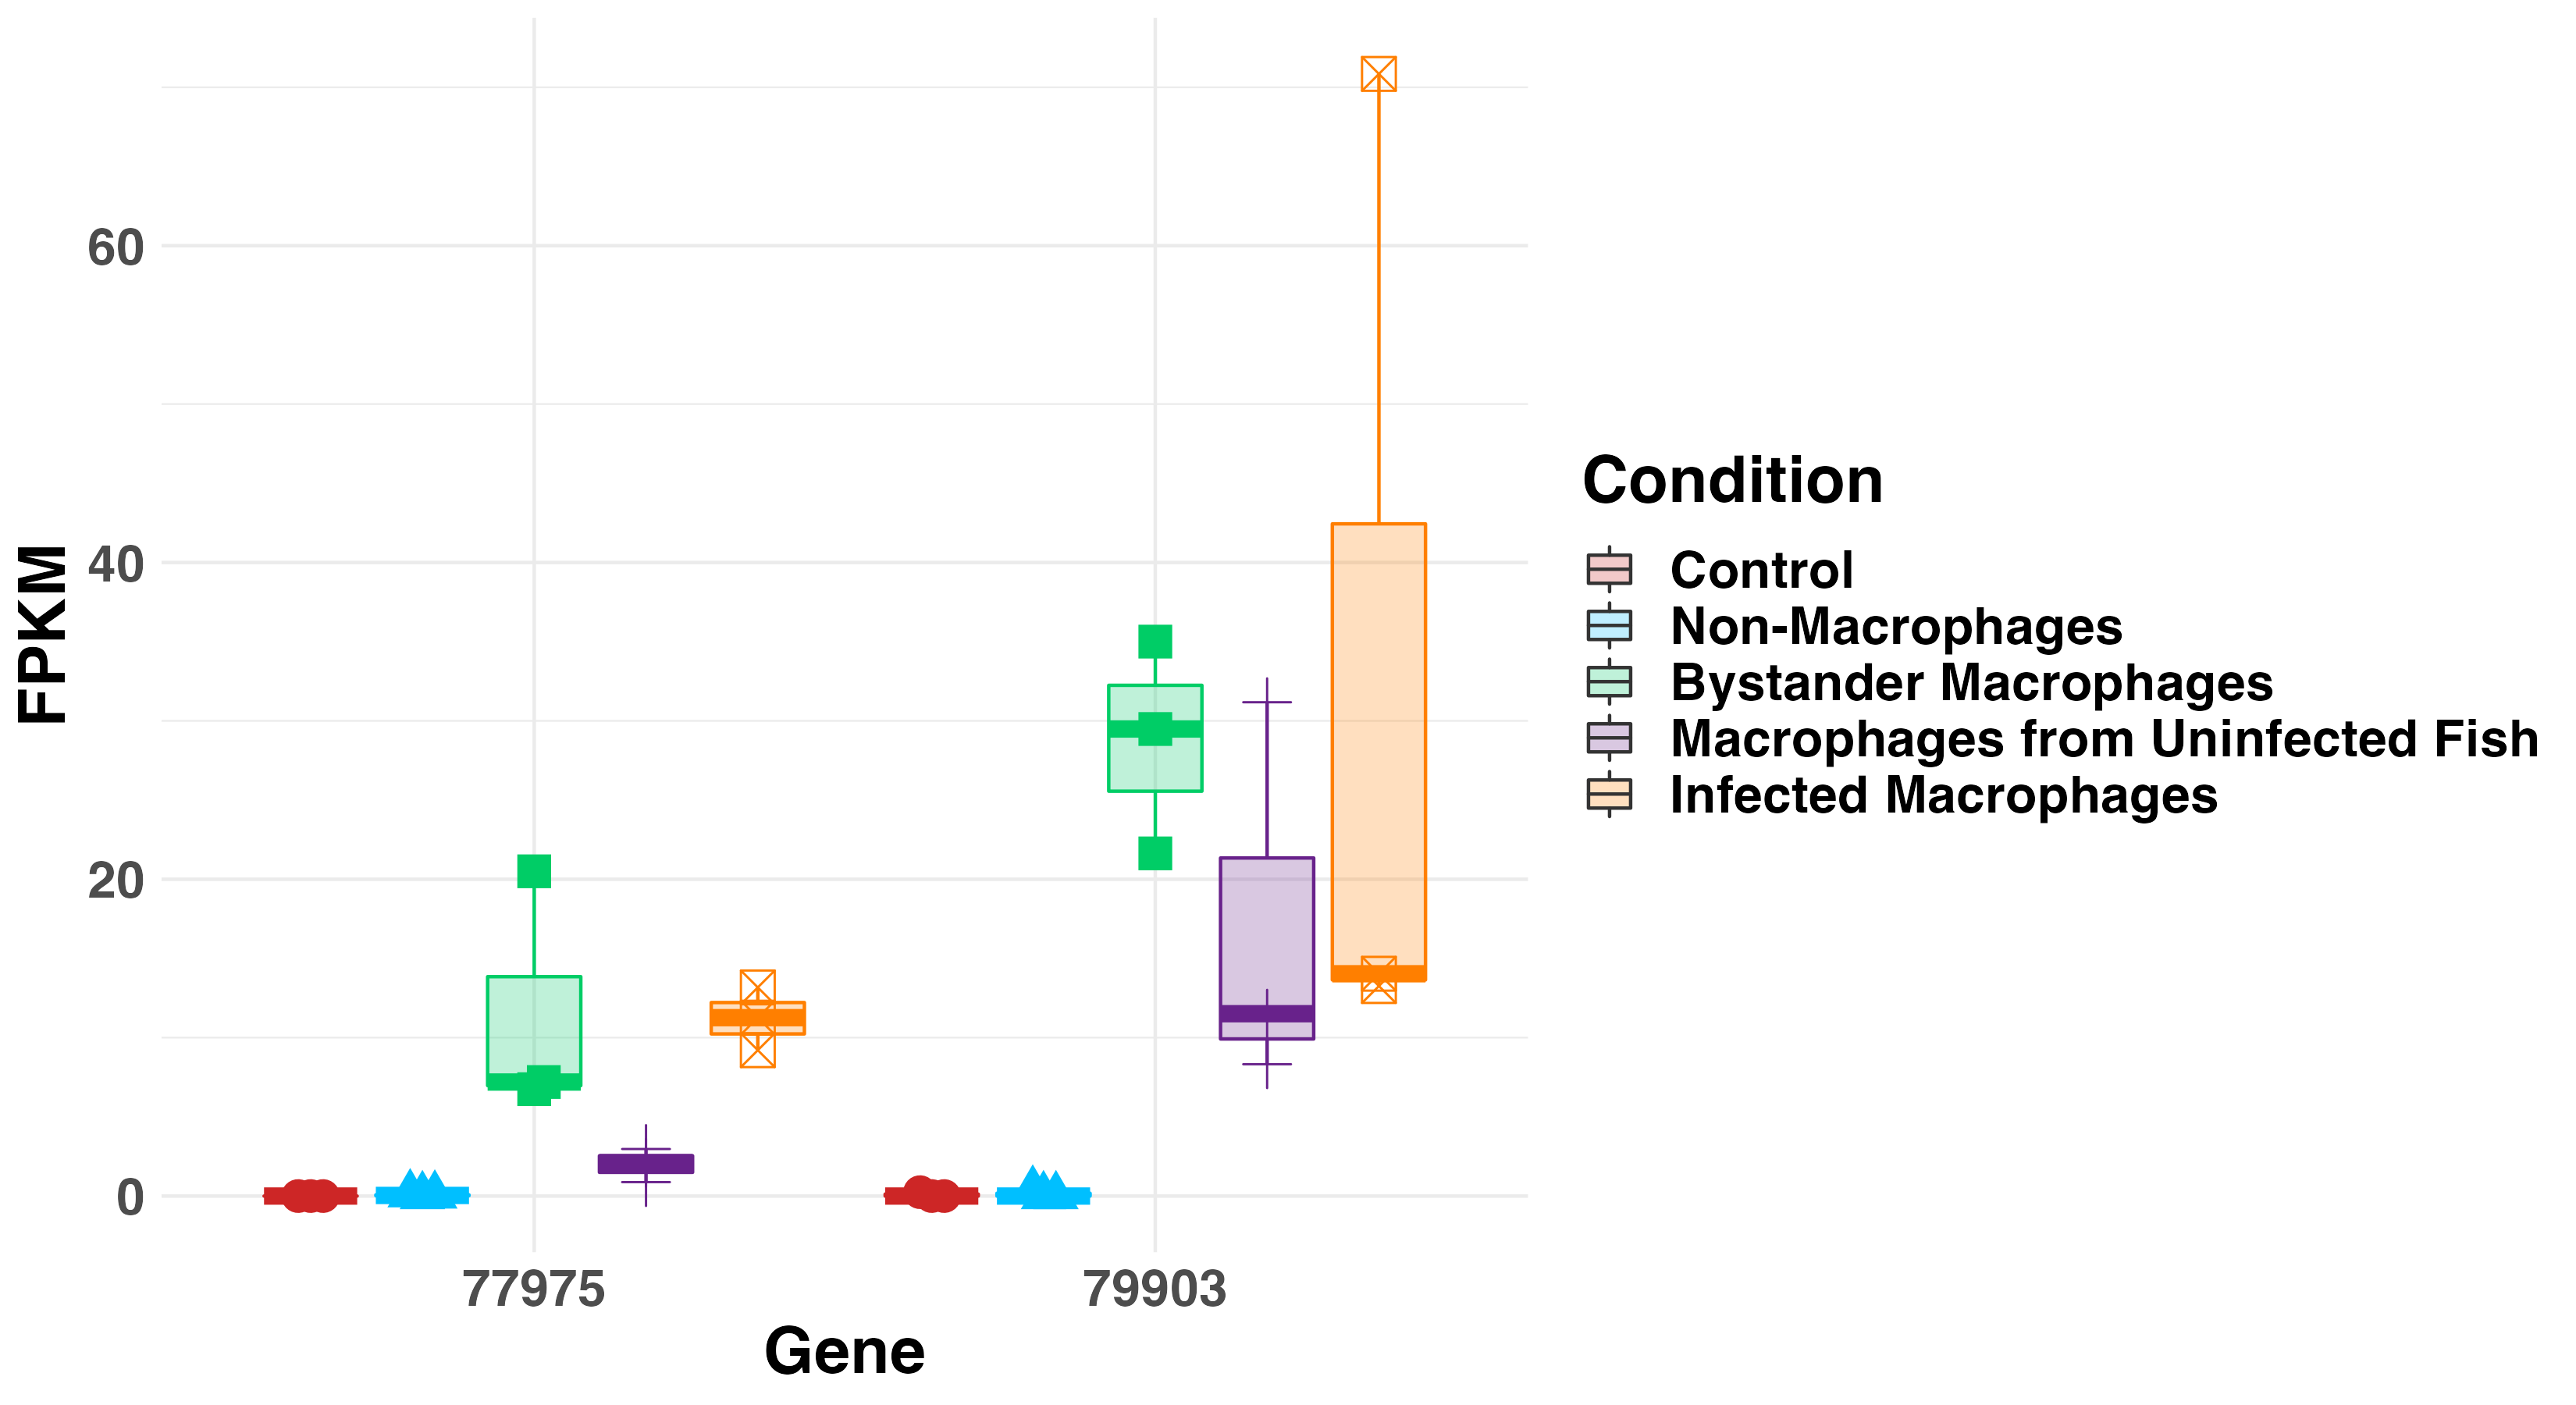
\includegraphics[width=\textwidth]{images/mincle_expression.png}
\caption{Comparison of the expression profiles of two of the putative MINCLE homologs, ENSDARG00000077975 and ENSDARG00000079903. Both of these genes are generally restricted to macrophages and are induced by the presence of mycobacterial infection, an effect exceptionally notable for 77975. This provides some evidence that these genes are regulated by mycobacterial infection and may be playing some role in this context.}
% Provide a label so we can cross-reference it from the tex
\label{figure:mincles}
\end{figure}

Additionally, it may be of some use to study the specific human MINCLE-mycobacteria interactions in the context of a whole immune system. Thus, going forward, it would be logical for future researchers to develop transgenic zebrafish that express human versions of MINCLE and MCL in macrophages and, perhaps, neutrophils, to assess the contributions of the human protein to conserved responses. This may also help to clarify some of the conflicting data in the literature around the role of MINCLE by using an overexpression model to capture the effect of excess MINCLE signaling. In the long term, gene replacement of the native MINCLE-like homolog with the human MINCLE would allow for a more authentically humanized model of macrophage biology within the zebrafish. Use of this as a complementing strategy if we can identify the zebrafish MINCLE would also serve as a more comprehensive humanized model to study the MINCLE-specific contributions to angiogenesis and bacterial control.

\singlespacing

\begin{center}
\begin{table}	
\caption{Putative zebrafish MINCLE homologs with key details about their native structure and mutants that have been generated thus far.}
\label{zfmincs} \tabularnewline
\vspace{0.5cm}
\begin{tabular}{|l|l|l|l|l|l|}
\hline
\thead{Gene ID} & \thead{Length (a.a.)} & \thead{CRD} & \thead{Similarity} & \thead{Mutation} & \thead{Site (a.a.)} \tabularnewline
\hline
56379 & 263 & kEPNn & 50.7\% & ::13 & 43 \tabularnewline
\hline
79903 & 263 & gEPNn & 53.3\% & ::13 & 207 \tabularnewline
\hline
77975 & 170 & gEPNn & 60.3\% & $\upDelta$8 & 108 \tabularnewline
\hline
\end{tabular}
\end{table}
\end{center}

\doublespacing

\section{Integration of Hypoxia Signaling}

The literature is replete with descriptions of HIF-1$\upalpha$ regulation of VEGFA production and signaling; the logical means by which to alleviate local hypoxia is through the recruitment of vasculature carrying oxygenated blood. This allows angiogenesis to occur when necessary and for the vasculature to remain quiescent under homeostatic conditions, where intravital oxygen concentrations are maintained at a high level. However, in areas of pathogen invasion, tumor growth, or tissue damage, the local oxygen concentration can fall, triggering the activation of the HIF-1$\upalpha$ signaling pathway. HIF-1$\upalpha$ is an oxygen-sensing protein that is expressed and rapidly degraded under normoxic conditions but stabilized under hypoxia. Under standard oxygen concentrations, two classes of regulatory proteins mediate prolylhydroxylation and proteosomal degradation of HIF-1$\upalpha$ in a process dependent on molecular oxygen.

Alternatively, HIF-1$\upalpha$ can be induced through transcriptional alterations in the homeostatic stoichiometry of HIF-1$\upalpha$ itself and the two families of regulatory proteins, PHD and FIH. This allow HIF-1$\upalpha$ to be induced under normoxic conditions, the presumed whole-body state of the zebrafish larva. This normoxia activation has been found to be important for myeloid immune responses, including those downstream of MINCLE activation, and may play an important role especially in the early signaling events of mycobacterial infection \citep{Nishi2008, Schatz2016, Schoenen2014, Thompson2017}. 

In the environment of the granuloma, both the host and pathogen must adapt to reduced oxygen tension. Mycobacteria can temporarily revert into a non-replicating state known as persistence, but this is not a viable strategy for long-term evolutionary success \citep{Ehrt2018, Stewart2003, Manabe2000, Pandey2008, zuBentrup2001}. However, during persistence, the bacteria are extremely difficult to kill as most antitubercular drugs are only effective on replicating bacteria \citep{Veatch2018}. Even during active growth, the bacteria and associated host cells must alter their metabolism to accommodate for reduced oxygen availability, with important consequences for host immunity \citep{Harper2012, Tsai2006, Prosser2017, Rustad2009, Galagan2013}. Despite our superficial knowledge about the importance and contributions of hypoxia in the lifestyle of \textit{M. tuberculosis}, we do not have a clear mechanism to genetically manipulate these responses or to differentiate the roles of hypoxia \textit{per se} from the activity of HIF-1$\upalpha$ signaling. Thus, going forward, new tools are going to be required to study not only the contributions of HIF-1$\upalpha$ in mycobacterial infections, but even more importantly, how those contributions intersect with the role of NFAT in inducing VEGFA production and angiogenesis in this environment.

\subsection{HIF for HIF's Sake}

\citep{Cardoso2015, Cramer2003, Dayan2008, Elks2015, Hammond2020, Kuhlicke2007, Li2021, Ogryzko2019, Santhakumar2012, Schild2020, Teran2022, Thompson2014}

Several groups, the most notable of which being Philip Elks's lab, have studied the contributions of HIF-1$\upalpha$ signaling to the immune response to mycobacterial infections, but there remain several needs as yet unaddressed. The Elks lab has utilized both dominant-negative and dominant-active versions of the zebrafish \textit{hif1ab} to modulate the activity of this pathway, particularly in neutrophils, and have found that activation of HIF-1$\upalpha$ prolongs inflammation and improve mycobacterial clearance, suggesting that at early time points, HIF-$\upalpha$ plays a protective role in infection \citep{Elks2011, Elks2013}. It was also found that HIF-1$\upalpha$ is important for the induction of TNF-$\upalpha$, which is a critical protective factor during infection \citep{Lewis2019, Flynn1995}. This work nicely complements work from Didier Stainier's lab, which used a combination of \textit{hif1aa} and \textit{hif1ab} mutant zebrafish and new macrophage-specific transgenic tools to manipulate the HIF-1$\upalpha$ signaling pathway and found that this pathway, specifically in macrophages, was critical for mediating developmental angiogenesis. Unlike the behaviors seen in neutrophils, specific expression of even a wild-type \textit{hif1ab} in macrophages was toxic to the cells and rendered them impotent \citep{Gerri2017}. This toxicity is likely due to sequestering of important binding partners, but may be due to metabolic changes that leave the cells unable to produce sufficient ATP, albeit by two divergent mechanisms -- wild-type \textit{hif1ab} may produce a strict reliance on glycolysis while dominant-negative \textit{hif1ab} may force oxidative phosphorylation at rates exceeding the ability to produce pyruvate. This evokes an important function of this pathway in these cells that current tools remain unable to address. 

To further the study of the HIF pathway in the context of mycobacterial infection, a set of new tools should be made: one is a set of reporter constructs to better identify both hypoxia and transcriptional induction of \textit{hif1ab} in macrophages and the other is a conditional approach to the expression of dominant negative and dominant active versions of HIF-1$\upalpha$ in macrophages, potentially enabling new cell-autonomous understanding of the role of this pathway in mycobacterial pathogenesis and angiogenesis.

Previous work in our lab using in situ hybridization for phd3 mRNA revealed the upregulation of this gene surrounding the mycobacteria, indicating hypoxia \citep{Oehlers2015}. The Elks lab generated a transgenic line using a bacterial artificial chromosome containing the promoter for \textit{phd3} that expresses GFP \citep{Santhakuma2012}, which serves as a useful spatial and temporal readout for HIF-1$\upalpha$ transcription factor activity across different tissues. However, this tool is unable to distinguish between normoxic and hypoxic activation or different cell types, so new tools are required to better address these questions.

During conditions of hypoxia, HIFs are degraded through hydroxylation in the oxygen dependent degradation domain (ODD) that contains two proline residues that are hydroxylated by PHD proteins, leading to proteasomal degradation. This ODD has been shown to be both necessary and sufficient to direct oxygen-dependent degradation, so it seems reasonable to use a macrophage-specific promoter to drive expression of ODD linked to a fluorescent protein as a reporter for granuloma hypoxia. This would be stabilized at low oxygen concentration while being constitutively degraded under normoxia. This would allow for a clearer report of the degree of present hypoxia and complement existing tools, including hypoxyprobe \citep{Cousins2016, Huang1998}.

In parallel, a reporter is needed to provide a readout of normoxic activation of HIF-1$\upalpha$, which is predominantly thought to be regulated at the transcriptional level. Therefore, either ectopic expression or direct protein fusion strategies would be appropriate to the study of this pathway. If some promoter could be identified that responded comparably to the native \textit{hif1ab} promoter or a CRISPR-mediated knockin could be generated, this would be a useful reporter of transcription-level induction of HIF-1$\upalpha$, a process likely relevant to inflammatory responses during infection.  This, in tandem with the previously mentioned ODD transgenes would allow for a more thorough dissection of the relative contributions of hypoxia \textit{per se} and the activity of HIF-1$\upalpha$.

As previous transgenic attempts have failed, the expression of dn-hif1ab and da-hif1ab in macrophages will require new approaches. It seems that misregulation of HIF-1$\upalpha$ results in some sort of developmental toxicity in the macrophage, so it is critical that HIF is only modulated in the time and place where it is most relevant. Thus, using established estradiol-responsive constructs, a set if fish should be made expressing dn-hif1ab and da-hif1ab covalently linked to ER50 degradation domains, which sequester proteins in the cytosol and target them for degradation except when in the presence of tamoxifen \citep{Miyazaki2012}. This would allow for the creation of HIF-modulating transgenes within macrophages that would be expected to have reduced toxicity and allow for time-targeted modulation of this pathway. Like the previous tools, this seems especially relevant in the context of mycobacterial granulomas from adult zebrafish, which are known to be hypoxic and more closely resemble human granulomas. These are likely to reveal not only new aspects of HIF modulation of angiogenesis, but broader impacts on the overall response to infection, especially given the central role of HIF-1$\upalpha$ in altering macrophage metabolism.

\subsection{Macrophage Metabolism in Immunity}

\citep{Biswas2012, Chawla2001, Corcoran2016, Covarrubias2015, Escoll2019, GalvanPena2014, He2021, Hong2004, Howard2020, Kelly2015, Langston2017, Mehla2019, Odegaard2011, OsadaOka2019, Palmieri2020, Phan2017, Qualls2016, Rabold2017, Russell2019, Somashekar2011, Stunault2018, Taylor2022, Viola2019, Wenes2016, Wilson2019, Yan2020, Yu2020, Kolliniati2022}

Upon activation, macrophages undergo a metabolic switch that corresponds, in part, to their longevity and function. While immediate-responding macrophages begin to utilize aerobic glycolysis for metabolism as a way to rapidly (albeit inefficiently) generate energy, longer-term macrophages utilize oxidative phosphorylation to optimize energy consumption over a long course of engagement \citep{Kiran2016}. Thus, while macrophages may initially use bursts of glycolysis to fuel rapid, oxidizing responses, this is unsustainable over the long term and these macrophages must either transition to the use of oxidative phosphorylation, disperse, or perish. These initial responses are regulated in part by the activation of HIF-1$\upalpha$. Wound sites and other sites of insult tend to have a reduced oxygen concentration, which drives this metabolic shift as well as the previously described induction of VEGFA to alleviate this hypoxia. 

The earliest events of the glycolytic switch in macrophages is triggered by the inducible nitric oxide synthase, which generates NO to inhibit mitochondrial respiration. The net effect is a reduction in oxidative phosphorylation capacity by the cell and a need for the utilization of an alternative mode of metabolism, which is supplied by glycolysis. Subsequently, HIF-1$\upalpha$ activation drives the transcription of glucose transporters and lactate dehydrogenase to block pyruvate utilization by the mitochondria. HIF-1$\upalpha$, as we have seen, also induces the expression of cytokines and chemokines, making it an integrated part of the overall response to detection of PAMPs, the model of which is LPS (see \autoref{lps}). As a major mediator of inflammatory responses, this glycolytic phenotype allows for rapid, energetically expensive response to immediate threats but is unsustainable over the long-term, leading to a shift back to oxidative phosphorylation.

\citep{ElKasmi2008}

In order to switch back to oxidative phosphorylation, HIF-1$\upalpha$ must be downregulated and alternate pathways induced; rather than nitric oxide synthase consuming cellular arginine to make nitric oxide and citrulline, arginase needs to be induced to produce urea and ornithine. Additional amino acid biosynthesis pathways also seem to contribute to the process of granuloma formation, but the precise roles of these are somewhat unclear. One of the issues with the study of mutants in discrete genes in these pathways is that much of this has been done \textit{in vitro} under the standard binary LPS or IL-4/IL-13 polarization conditions or in the mouse, where more comprehensive profiling is possible but the knockout of \textit{Arg1} or \textit{Nos2} might not fundamentally change the cellular identity of these populations although it may shift them on the M1-M2 dichotomy by the formal definitions. Nevertheless, the relative contributions of HIF-1$\upalpha$ to the metabolic state of the macrophages depends on the interplay of formal hypoxia as well. 

Under sustained immunological stimulation in hypoxia, such as that found in a tuberculous granuloma, metabolic reprogramming toward oxidative phosphorylation still occurs in macrophages. The conflict between the production of VEGF, the M2-like identity of many granuloma macrophages that express VEGF, and the downregulation of HIF-1$\upalpha$ in M2 macrophages raises important questions about the factors that were presumed to be regulating VEGF production prior to the present work, which presents the alternative model of a C-type lectin receptor-NFAT transduction pathway able to induce VEGF. It may be that, under this model, that the metabolic status of the macrophages is unimportant for VEGF production, although this would be, to some degree, in contradiction with other parts of the literature. A further mystery is why VEGFA is so frequently considered an M2 cytokine when its transcription was thought to be dependent on HIF-1$\upalpha$, a gene induced under M1 conditions. A more thorough integration with the findings of this work with the general metabolic status of granuloma macrophages that produce VEGF normally will be important for resolving some of these quandaries on the contribution of HIF-1$\upalpha$ to granuloma macrophage metabolism, antibacterial responses, and angiogenesis.

\subsection{HIF-NFAT Interactions}

A tempting hypothesis is that HIF-1$\upalpha$ and NFATC2 are regulating one another to induce the expression of VEGFA. The model most consistent with the existing literature is that NFATC2 is upregulating the transcriptional expression of HIF-1$\upalpha$ under circumstances where HIF-1$\upalpha$ is already being stabilized. This would feed-forward the induction of VEGFA and may be essential for regulating these responses in normoxic environments or very early in infection. 

A piece of standalone support for this model is a study conducted in mast cells that demonstrated a calcineurin-NFAT dependent upregulation of HIF-1$\upalpha$ at the transcriptional and protein levels. Treatment of these mast cells with ionomycin, which increases cytosolic calcium concentrations, caused these effects in a way that was able to be inhibited by tacrolimus treatment. Additionally, this effect was exacerbated by culture under 1\% O\textsubscript{2}, a description that corresponds well to the behavior of NFATC3 in the myocardium, where hypoxia increased expression of endothelin-1 in a way that is sensitive to superoxide and the activity of NFATC4, which can also be activated by hypoxia \citep{deFrutos2011, RamiroDiaz2014, Moreno2015}. Additional studies found that hypoxia activated NFATC3 to promote pulmonary smooth muscle proliferation in a way that might promote pulmonary hypertension \citep{Hou2013}. Hypoxia can also increase proliferation of human fibroblasts through NFATC2 independently of HIF-1$\upalpha$ but dependent on HIF-2$\upalpha$ \citep{Senavirathna2018}. None of these studies but the last investigated a mechanism to integrate this activation of NFAT under hypoxia with the roles of HIF-1$\upalpha$ despite these phenotypes having been previously described to correspond with HIF-1$\upalpha$ activity \citep{Cui2021, Qi2017, Li2014, Thackaberry2002, SonanezOrganis2016}. Even the \citeauthor{Senavirathna2018} only investigated this effect within a relatively limited scope (proliferation) and not in respect to the diversity of phenotypes that are stimulated by hypoxia.

To study these interactions, it seems that combinatorial chemical inhibition strategies could be utilized, although HIF-1$\upalpha$ inhibitors are relatively sparse in number and understudied \citep{Viziteu2016}. However, this would only scratch the surface in pursuit of epistatic interactions between these proteins and would neglect the potential for protein-protein interactions in mediating part of the effect. A structure based approach targeting known interacting domains on HIF-1$\upalpha$ and its DNA binding domain may reveal important transactivation role for HIF-1$\upalpha$ as well as resolve some questions about the direct versus indirect nature of NFAT regulation of hypoxia responses. Much of this work could be done in a heterologous model (HEK-293T cells, for instance) to more efficiently assess these types of binary interactions. Larger scale screening approaches by two-hybrid would be another potential avenue for such a project to go as the interacting partners of various domains of NFATC2 remain only partially resolved. Proximity ligation approaches, which will be discussed moreso later on, offer another possibility for dissecting the HIF-1$\upalpha$ interactome. Unfortunately, the state of reagents to work with toward these ends in the zebrafish are somewhat limited and additional groundwork would be required to study some of these processes in an \textit{in vivo} context, although this seems like an excellent direction for a future Ph.D. project.

\section{Cotranscriptional Interplay}

To further dissect the contributions of other transcription factors to the NFAT-dependent angiogenesis response, we can make use of our THP-1 macrophage platform to study the role of NFAT interacting partners in the overall response to \textit{M. tuberculosis} exposure. While wild-type NFATC2 is able to interact with a panoply of other transcription factors through both C- and N-terminal domains, the domains important for particular binary interactions have been teased out over time, largely by Anjana Rao's lab. Thus, to simultaneously test the sufficiency of NFATC2 in inducing transcriptional responses, the importance of AP-1 transcription factor binding, and the ability for NFATC2 itself to bind DNA, I have developed a set of expression plasmids that drive expression of the following:

\singlespacing

\begin{center}
\begin{table}[h]
\caption{Lentiviral expression constructs to assess the role of NFATC2 domains for induction of VEGFA signaling.}
\label{table:canfat} \tabularnewline
\vspace{0.5cm}
\begin{tabular}{|p{2in}|p{3in}|}
\hline
\thead{Plasmid} & \thead{Utility} \tabularnewline
\hline
pLEX:mPapaya & Empty expression vector driving expression of only the conjugated fluorescent protein, for background comparison. \tabularnewline
\hline
pLEX:CA-NFAT1 & Expression of a constitutively active NFATC2 that drives transcriptional responses independent of calcineurin. \tabularnewline
\hline
pLEX:CA-NFAT1-$\upDelta$DBD & Expression of a constitutively nuclear NFATC2 that is unable to bind DNA, to assess the contributions of NFAT binding on the induction of VEGFA. \tabularnewline
\hline
pLEX:CA-NFAT1-$\upDelta$RIT & Expression of a constitutively active NFATC2 unable to interact with AP-1 transcription factors, to determine the contribution of this family to the VEGFA response. \tabularnewline
\hline
pLEX:CA-NFAT1-$\upDelta$DBD-$\upDelta$RIT & Expression of a constitutively nuclear DNA binding domain mutant also unable to interact with AP-1 transcription factors. \tabularnewline
\hline
\end{tabular}
\end{table}
\end{center}

\doublespacing

These plasmids will enable a genetics-first dissection of the activity of NFATC2 and its potential sufficiency to induce transcription of VEGFA. While, as noted in \autoref{pap:disc} and seen in \autoref{fig:nfatpro}, the VEGFA promoter has a number of putative NFAT binding sites, the activity of these remains unknown. Using these new genetic tools in the defined environment of THP-1 macrophages it should be possible to dissect the function of these sites. Distant future approaches may utilize deeper genetic probing to identify particular sites of especial importance, as has been done in \citet{Chang2004}. While that publication found one site that was bound by NFAT in the myocardium, the particular binding site of importance may vary by cell type and circumstance. 

It is also possible that non-AP-1 transcription factors are important for NFAT activity and this is a trickier proposition to address, but could be done through either immunoprecipitation-mass spectrometry or biotin tagging approaches via BioID \citep{Roux2012}. The advantage of the former is the identification of more stable interactions and could be done in tandem with DNase-seq, ChIP-seq, or ATAC-seq to identify promoter occupancy of this isoform. The latter may be a technically less challenging approach, however, and may provide a useful readout of the total set of interactions experienced by NFATC2 over the course of $\upgamma$Mtb exposure. The former can also be done in genetically unmodified cells while the latter would require some (minimal) additional cloning and generation of yet another lentivirus for the purpose of tagging NFATC2 with one of the several biotin ligases now available \citep{Cho2020}. Both seem useful and complementary and should be considered going forward to more comprehensively understand the NFAT interactome during mycobacterial infections. I hypothesize that there are as-yet unobserved protein-protein interactions between NFATC2 and HIF-1$\upalpha$ that would potentially shed light on the transcriptional regulation of VEGFA in diverse contexts including in cancer and autoimmunity. 

\subsection{NFAT:AP-1 Interactions}

\citep{Boise1993, Eferl2003}

The most exhaustively studied transcriptional partner for NFAT is the AP-1 transcription factor superfamily, which includes proteins in the JUN, FOS, ATF, and MAF families. While some of these may strike the reader as being critical regulators of cell growth and tumorigenesis, they also play critical roles in other aspects of normal biology including in immune responses \citep{Macian2001}. AP-1 binding sites are often adjacent to NFAT binding sites and these two transcription factors\footnote{To avoid providing unnecessary amounts of detail, I will refer to AP-1 as a monolithic "transcription factor" much of the time. While each of the proteins in this family serve different functions, the subtleties are perhaps beyond the scope of this prospective overview. The guiding question of this section -- is an AP-1 transcription factor cooperating with NFAT to drive VEGFA transcription -- is sufficiently broad that future experimentation would almost certainly eventually seek to identify, at the gene level, which is responsible.} may cooperate to drive the transcription of VEGFA. These cooperative interactions may be close in proximity or over a long distance and may be direct protein:protein interactions or more indirect. Regardless, given the imminent importance placed on NFAT:AP-1 interactions, this seems to be an excellent place to start on a targeted list of potential interacting partners.

A few approaches can be taken. The first, utilizing the previously described pLEX:CA-NFAT-$\upDelta$RIT constructs, would give an indication about the importance of direct interactions with NFATC2, as these mutate the critical residues for complexing with AP-1 proteins. Additionally, there are a number of relatively broad inhibitors against AP-1 that could be used to test whether inhibition of AP-1 alone alters the VEGFA transcriptional response to mycobacteria \textit{in vitro} or the overall angiogenic response \textit{in vivo} \citep{Makino2017, Huang1997}. It has been previously demonstrated that AP-1 can activate VEGFA transcription as well as VEGFD, suggesting that this pathway may have as-yet unappreciated roles in inducing VEGFA during immune responses and may act in concert with NFAT to execute these functions\footnote{More classical data suggests that HIF-1$\upalpha$-dependent VEGF upregulation is independent of AP-1, although this data may be limited by the scope of the time and the particular experimental conditions. Or hypoxia-induced VEGFA may be independent of AP-1, but pathogen-induced VEGFA is dependent on it -- these all remain to be explored \citep{Finkenzeller1995}.} \citep{Shih2001, Debinski2001, Wang2016, Josko2004, Guo2022}.

\subsection{NFAT:NF$\upkappa$B}

\citep{Fisher2006, Liu2012, LopezRodriguez2001, Zhao2015}

As has been discussed previously (see \autoref{}), the interplay between NFAT and NF-$\upkappa$B is widely discussed but the precise biological consequences of these two transcription factor families in inducing VEGFA remain unknown. It has previously been shown that NF-$\upkappa$B is able to induce the transcription of VEGFA in various contexts \citep{Xie2010, Greenberger2010, Lukiw2003} and is important for VEGFA expression in macrophages \citep{Kiriakidis2003}. citet{Lukiw2003} even uncovered important interactions between HIF-1$\upalpha$ and NF-$\upkappa$B in the induction of VEGFA during hypoxia, suggesting the potential for there to be multiple layers of signaling required to induce VEGFA during particular context and which may vary based on the stimulus.

The overarching theme in studies of NFAT-NF-$\upkappa$B interactions is that they can either be antagonistic or cooperative and \textit{a priori} prediction of which is likely to occur has been elusive \citep{Khalaf2013}. Foundational studies at addressing found cooperative roles for NF-$\upkappa$B and NFAT in regulating the expression of IFN-$\upgamma$ \citep{Sica1997} and that they were differentially induced by alterations in cellular calcium \citep{Dolmetsch1997}. And as we have seen in the context of osteoclast biology, NF-$\upkappa$B can bind to the promoter of NFATC1\footnote{The relevance to other NFAT proteins remains unknown, but at least NFATC2 has putative NF-$\upkappa$B binding sites in the proximal promoter.} to drive increased expression to allow for osteoclast differentiation \citep{Asagiri2005}. And in the context of TLR agonism, NFATC3 nuclear occupancy was important for NF-$\upkappa$B responses but was not induced by TLRs and could either enhance or inhibit NF-$\upkappa$B responses \citep{Minematsu2011, Conboy1999}. Competitive promoter occupancy and yet other regulatory factors may be involved in regulating these roles, but this serves as an interesting potential regulatory mechanism worthy of investigation in the context of macrophage VEGFA signaling given the composite evidence of NF-$\upkappa$B importance for macrophage expression of VEGFA and the known layers of regulation surrounding NFAT and NF-$\upkappa$B signaling.

One of the interesting observations that came out of the work studying the NFATC2-dependent transcriptional responses to \textit{M. tuberculosis} was the observation that $\upgamma$\textit{Mtb} exposed THP-1 macrophage seemed to have greater production of NFATC2 protein by immunofluorescence, an unusual potential regulatory mechanism only rarely described in historical literature \citep{Asagiri2005, Aramburu1995} and then only for NFATC1. The concept that there may be some sort of upstream priming event that stimulates NFATC2 production and/or downregulation of NFATC2 protein degradation offers the potential for a new layer of regulation of NFAT activity. Further experimentation will need to be done to confirm this and I would propose RNA-seq as an excellent first-attempt to categorize some of the macrophage-specific responses to extracellular exposure to \textit{M. tuberculosis}. 

\section{New Genetics Tools for the Study of NFAT Signaling}

One of the dominant tools in the field for the study of intracellular calcium flux is the use of GCaMP, a modified green fluorescent protein that fluoresces in response to calcium binding \citep{Nakai2001}. Since its initial development, many interactions have developed allowing for ever-finer detection of various aspects of cellular calcium concentrations and localization. These tools have been used in the fish to detect and manipulate cellular behavior in both fixed and freely moving fish \citep{Beerman2015, Kim2017}. These tools have clear promise in better understanding the biology of NFAT activation, but likely need tethering to either the channels or proteins themselves or a specific cellular compartment to increase spatial resolution; a whole-cell approach is no longer sufficient for the proper understanding of NFAT activity in this context and finer resolution would greatly aid in the identification of future mechanisms. Given findings from \citet{Kar2015} on the importance of nuclear calcium in regulating the activity of at least NFATC3, it would be beneficial to have new tools to monitor these alterations in real time. 

An initial approach would take advantage of some of the new technologies available in the zebrafish (reviewed in \autoref{newtech}) by generating an endogenously GCaMP-tagged \textit{nfatc2a} in the zebrafish to monitor the timing of calcium flashes and how those correspond to the activation state of the protein, able to be visualized by intercompartmental trafficking. By using high temporal and spatial resolution imaging offered by LightSheet \citep{Reynaud2008}, it would be possible to monitor on the seconds resolution the activation status of Nfatc2a within macrophages in response to mycobacterial infection. This finely tuned reporting behavior would reveal key details about the timing and kinetics of NFAT activation during infection and how that activation corresponds to the induction of \textit{vegfaa} and angiogenesis.

In the long-term, it is likely to be worth exploring the possibility of generating a floxed \textit{nfatc2a} allele to allow study of this protein in a particular cellular context. While the use of VIVIT allows for gross examination of NFAT-dependent phenotypes, it would be beneficial to be able to study individual isoforms' contributions to given phenotypes. This is technically already possible, but is rather laborious. Should newer approaches to the generation of knock-in zebrafish lines emerge, this should be a foremost consideration in the continuation of this work.

It will also be interesting to start teasing out non-macrophage cellular contributions to angiogenesis. While we have already seen that depletion of macrophages reduces the angiogenic phenotype in response to mycobacterial infection \citep{Oehlers2015}, it is not known if other cells types may be able to compensate at other stages of infection. Thus, we could apply the \textit{irf8\textit{st95}} fish line, which lacks macrophages due to loss of a transcription factor essential for macrophage development, to study these processes in the larva and the adult \citep{Shiau2015, Xu2012, Tamura2005}. Ambitious approaches would incorporate reconstitution of the macrophage population in an otherwise wild-type \textit{irf8\textit{st95/st95}} with \textit{nfatc2a} macrophages to more precisely identify the requirement for these cells in angiogenesis. A slightly simpler approach would adopt the strategy used by \citet{Cronan2021} to conduct whole kidney marrow transplantation into \textit{myb} mutant larvae, reconstituting the entire hematopoietic system with \textit{nfatc2a} mutant cells. Any of these approaches should allow for deeper study of macrophage NFATC2 biology in the zebrafish model.

\section{Mycobacterial Interactions with Other Aspects of Vascular Biology}

The focus of the present work has been on a rather coarse readout of vascular biology: angiogenesis or not. However, as was discussed briefly in \autoref{angiogenesis}, the biology of the endothelium is far more complex than just sprouting angiogenesis and the interaction of the granuloma with the vascular is more complex as well. This makes it imperative to develop a more nuanced understanding of how these other factors may contribute to the pathology of the disease and how NFAT signaling may modulate these factors as well. 

A radical approach that may be of some utility in addressing some of these more challenging questions would require the development of a new model wherein \textit{ex vivo} cultured granulomas are co-cultured with endothelial cell lines to start addressing some of the contributions of different genetic factors to the ability of the granuloma to alter endothelial cell biology more directly. While it is known that human umbilical vascular endothelial cells (HUVECs) can respond to zebrafish Vegfaa, it may be worthwhile to explore a more native model. Endothelial cell lines from other fish species have been established and it could be of great utility to explore the possibility of establishing something similar for the zebrafish \citep{Pham2017, Luque2014}. A genetically tractable system for generating these lines would allow for both granuloma-derived signals and endothelial responses to be measured in a more tightly controlled environment. Given many of these objectives involve more cell biology than simply the growth of vessels, the ability to observe them in greater isolation may prove necessary if these are to be effectively addressed.

\subsection{Vascular Permeability}

\citep{Akwii2021, Augustin2009, Huang2010, ParkWindhol2016, Saharinen2017, Thurston2012}

A previous study from the Tobin lab found that angiopoietin signaling was a critical mediator of vascular permeability during mycobacterial infection, a finding consistent with that of tumors, where ANG2 signaling induces alterations in the biology of the endothelium through TIE2 \citep{Oehlers2017, Duran2021, Goel2012}. Inhibition of angiopoietin signaling resulted in a reduction in bacterial burden and improved vessel normalization. However, more recent findings have noted that granuloma macrophages do not seem to be a major source of angiopoietins\footnote{This is at least true of the 14 days post infection time point at which the samples were taken and similar findings can be found from \citet{Gideon2022}.}, which creates a bit of a conundrum: if we know that these genes are expressed during infection and play a role in the overall course of disease, where are they coming from? \citep{Cronan2021} 

Angiopoietin signaling is a complex affair, with multiple ligands and receptors, but the focus is centered on the bifunctional ligand, angiopoietin-2 (ANGPT2 or ANG2) and the receptor TIE2\footnote{TIE1 primarily plays a complementary role with TIE2 as a heterodimer -- this is a bit beyond the present topic but for further reading, \citet{Savant2015} and \citet{LaPorta2018} have excellent studies on how TIE1 contributes to angiogenesis in development and cancer.}. While at homeostasis ANG2 can activate TIE2 to promote vascular stability, but in the context of inflammation, it becomes antagonistic through combinatorial effects with various cytokines, and induces vascular permeability. This leakiness results in a disregulated vascular environment that promotes tumor and, seemingly, bacterial growth; normalization with antibodies induces vascular regression and exerts anti-tumor effects. This also implicates ANG2 as an important mediator of angiogenic processes in concert with VEGF. It is known that endothelial cells can produce their own ANG2 to signal in an autocrine and paracrine manner as part of normal vascular biology. Additionally, stromal cells in nearby tissues can respond to a cytokine environment and induce the expression of ANG2. This provides neighboring cells and the endothelium itself an important role in regulating endothelial biology and may be at play in the context of the granuloma.

If nearby fibroblasts, pericytes, or the endothelium itself are producing ANG2, as would be suggested by \citet{Gideon2022}, then we are missing out on crucial aspects of stromal-granuloma interactions in the dataset from \citet{Cronan2021}. What gene networks might be regulating these processes and are macrophages a major source of a key inducing cytokine(s)? These are difficult questions to address with existing tools and the gene duplication of the zebrafish presents fresh difficulties. Others in the lab have developed CRISPR-Cas9 mutations in zebrafish \textit{angpt2a}, \textit{angpt2b}, and \textit{tie2}, which may be useful in dissecting some of these effects. Studies using these lines and, potentially, the development of novel \textit{angpt2} transgenic reporters would help to narrow on the cellular identity of ANG2-producing cells in the granuloma and how modulation of those cells could offer an alternative pathway toward vascular normalization in the granuloma either independent of or in concert with VEGF-targeting therapies. As we have seen with bevacizumab, it will likely be necessary to develop a multi-pronged approach to vascular targeting and a more thorough study of this pathway during mycobacterial infection would constitute a major contribution in that direction. An unlikely, but plausible, hypothesis would be that NFAT in macrophages is regulating the production of a cytokine that is stimulating ANG2 production by fibroblasts or pericytes. Such an intercellular signaling network would be a fascinating new aspect of granuloma angiogenesis biology.


\subsection{Pericytes}

\citep{Correa2014}
\citep{ClaessonWelsh2015}
\citep{Eklund2017}
\citep{Hato2008}
\citep{Sakamoto2010}
\citep{Keskin2015}
\citep{Shin2016}

\subsection{Extracellular Matrix}

Although this dissertation has not particularly addressed the biochemistry of the focal chemokine -- VEGFA -- it is an intriguing protein with multiple layers of regulation, including the existence of multiple splice variants. The two major ones VEGFA\textsuperscript{121} and VEGFA\textsuperscript{165} have distinct capacities for binding to the extracellular matrix (ECM), with VEGFA\textsuperscript{165} binding to heparin while VEGFA\textsuperscript{121} freely diffuses through ECM. 

\subsubsection{Tetranectin}

\subsection{Other Angiogenic Stimuli}

\citep{Jeon2007, Liu2014, Sugden2017, Ubil2014, Wu2007}
\citep{Correa2014}

\section{Lymphangiogenesis}

This project has focused strictly on the proliferation and growth of vascular endothelial cells during mycobacterial infections, a process known as angiogenesis. However, a parallel process exists concerning the lesser studied lymphatic vascular system and this is known as lymphangiogenesis. The evolutionary segregation of blood and lymph circulation has led to distinct but very closely related mechanisms of regulation during development and pathology, which suggests a potential role for this pathway during tuberculosis infection as well. While this process is less extensively studied, it is a critical component of the vascular development of vertebrate organisms and is essential for proper fluid homeostasis and immune system function, as lymphatic vessels are the route along which antigen presenting cells "drain" into the lymph nodes to prime the adaptive immune system. Failures of lymphangiogenesis result in lymph\oe dema and general problems with fluid balance \citep{Makinen2001}. In the context of disease, the lymphatic system is essential for proper immune behavior, but during chronic conditions like cancer or tuberculosis, lymphangiogenesis can be subverted by the insult for their own benefit. In cancer, lymphangiogenesis is utilized to provide additional routes of metastasis away from the primary tumor; the role in tuberculosis is comparatively less well studied.

Lymphangiogenesis is primarily mediated through an analogous set of ligand-receptor pairs to that seen in hemangiogenesis. VEGFC and VEGFD\footnote{At least VEGFD acts non-redundantly and is also able to stimulate hemangiogenesis in the zebrafish and, given the findings presented in \autoref{cancerang}, both of these likely to play roles in other angiogenic processes \citep{Bower2017a}.} are major pro-lymphangiogenic chemokines and bind VEGFR3 on the lymphatic endothelium to stimulate lymphangiogenesis \citep{Alitalo2005, Kuchler2006, Haiko2008}, a process which depends on functional ERK signaling, much like hemangiogenesis \citep{Shin2017}. During development, a portion of the cardinal vein differentiates into lymphatic progenitors \citep{Yaniv2006, Nicenboim2015} and begins to elaborate into a full lymphatic system by approximately 3 days post fertilization in the larval zebrafish; these budding vessels are guided by arterial cues, which allows much of this system to parallel the blood endothelial system \citep{Jung2017, Bussmann2010}. This process ultimately leads to a complete lymphatic system able to drain excess fluid and remove insults from within tissues, although zebrafish are not known to possess lymph nodes as mammals do and the primary sites of antigen presentation lie elsewhere \citep{vanLessen2017, Onder2017}.

During cancer growth, the tumor itself and the tumor associated macrophages that surround it both contribute to lymphangiogenesis, which provides a means of dissemination for the tumor to distal body sites. Lymphangiogenesis and VEGFC/D can facilitate metastasis in the tumor although it is not clear whether this mechanism operates solely through induction of lymphangiogenesis or if VEGFC/D can act directly on the tumor itself, analogously to VEGFA autocrine activity \citep{Stacker2014}. The primary site of initial metastasis -- to the lymph node -- is a symptom of the lymphatic involvement in this disease. Of course, it was conceptually possible that the lymphatic endothelium was a bystander, but it is clear that the lymphatic system active grows and remodels in response to tumor signals. It has since been demonstrated that VEGFC overexpression by cancer cells in the tumor drives increases lymphangiogenesis and early lymph node metastasis, implicating active manipulation on the part of the tumor in this \citep{Duong2012}. Several different tumors also overexpress the lymphangiogenic effector CCBE1, which aids in processing VEGFC into its active form to potentiate lymphatic growth \citep{Hogan2009, LeGuen2014, Li2018b, Song2020, Zhao2018}.

Tumor-associated macrophages have been linked to this process through tumor-directed activation of the inflammasome that drives IL-1$\upbeta$ processing to increase lymphangiogenesis \citep{Weichand2017}. This interesting mechanism provides the tumor multiple means of inducing a full spectrum of different signals that facilitate its spread. Macrophages more broadly also play key roles in the induction of inflammatory lymphangiogenesis, also partially mediated by IL-1$\upbeta$ as well the induced expression of VEGFC and VEGFD during insult. After tissue damage, it is critical to direct the growth of new lymphatic vessels toward the injury in order to facilitate drainage and immune access, but excessive lymphatic inflammation is harmful. An additional mechanism that macrophages can use to induce lymphangiogenesis is through IL-33 production, which induces a complex intracellular cascade that include nitric oxide signaling to drive inflammation \citep{Han2017}. Similarly, TNF-$\upalpha$ has been shown to induce lymphangiogenesis by stimulating production of VEGFD\footnote{Could it be through NFAT? Perhaps and if so that would add another putatively positive aspect to targeting this pathway.} \citep{Hong2016}. Conveniently, the zebrafish is able to be utilized to model many of these processes in inflammatory lymphangiogenesis, allowing us to adapt it to the study of these processes in mycobacterial infection \citep{Okuda2015}.

To date, there have been two major sets of studies on the role of the lymphatic system in mycobacterial infection, which is a relative indictment on the attention that has been paid to this potentially significant contributor to disease. The first, from \citet{Harding2015}, examined this pathway through chemical inhibition to block VEGFR3 activity. This study found that reduction of lymphangiogenesis resulted in decreased proliferation of \textit{M. tuberculosis}-specific T cells, suggesting that lymphangiogenesis blockade reduced access of antigen-presenting cells to the lymph nodes to stimulate T cell proliferation. However, this was done in the context of BCG infection, so the effects on bacterial burden were unable to be ascertained. Future studies on this pathway during infection with virulent \textit{M. tuberculosis} seems to be in order as well as a more thorough examination of the consequences of this on disease progression over time. While blocking lymphangiogenesis may alter the ability of the immune system to generate a robust adaptive response, it may also alter cellular dynamics earlier in infection in host-beneficial ways, but these things are currently unknown. A synthesis of the larval and adult models of zebrafish infection seem to be promising methods for assessing some of these impacts.

The second studies interrogated the function of lymphatic endothelium as a replicative niche for \textit{M. tuberculosis} \citep{Lerner2016, Lerner2020}. Although tuberculosis is classically a pulmonary infection and the pulmonary niche is the only effective route of transmission, the most common extrapulmonary presentation of tuberculosis is in the lymph nodes, a disease known from antiquity as scrofula. The infection of the lymph nodes implied that the bacteria had a productive replicative niche in the lymph nodes, which could have simply been macrophages, but this study found that mycobacteria could directly infect the lymphatic endothelium \citep{Lerner2016}. Indeed, it appears that lymphatic endothelial cells are a relatively permissive host cell type, as the bacteria will cord within these cells as a mechanism of host immune evasion \citep{Lerner2020}. This highlights a binary role for lymphangiogenesis during infection, where it may be important for priming certain adaptive immune responses, but may also offer a convenient replicative niche; the net effect remains in need of study and the zebrafish may offer an ideal model in which to do so.

There are an abundance of tools in the zebrafish to study lymphangiogenic processes. The \textit{lyve1} transgenic lines allow for visualization of lymphatic vessels throughout life, where they appear at approximately 3 days post fertilization \citep{Okuda2012}. This allows both larval and adult zebrafish to be used to study these processes, unlocking the full spectrum of disease. Additionally, a number of genetic tools exist to allow for study of this process. Notably, the \textit{hsp70l}:\textit{sFlt4\textsuperscript{bns82}} line is able to potently inhibit the generation of lymphatics through overexpression of a soluble decoy VEGFR3 \citep{Matsuoka2016}. Together, these lines can offer both a means of visually assessing the state of the lymphatic endothelium as well as block lymphangiogenesis at various time points. Pioneering studies should evaluate the degree of lymphangiogenesis induced by \textit{M. marinum} infection and, thorough genetic inhibition, study the role of this at both early and late stages of infection in the larva and the adult. It is my hypothesis that, especially in the adult, there is extensive lymphatic involvement that contributes to infection and, like previous studies, may provide an extragranulomatous replicative niche during earlier stages of infection \citep{Lerner2016}. The ability to study the contributions of lymphatics within a model that presents with necrotic, epithelioid granulomas offers the opportunity to also evaluate them as a potential route of dissemination complementary to hematogenous dissemination. 

There are several proposed strategies to block lymphangiogenesis in these diverse contexts. One is, of course, through pharmacological inhibition of VEGFR3 signaling in a manner analogous to that of bevacizumab, but this may be subject to subversion through compensatory VEGFR2 signaling. Another is to block aspects of the lymphatics that are required for growth, such as integrin $\upalpha$5 \citep{Dietrich2007} or fatty acid oxidation \citep{Wong2017b}. The future of this remains uncertain, although these drugs may act as excellent adjuvants to existing antihemangiogenic therapies.

\section{Generalizability}

One of the major questions is whether or not the findings I have shown in \autoref{chap3} are able to be generalized to other disease contexts. The most notable possibility is in cancer, where tumor-associated macrophages are well known to produce VEGFA to induce tumor angiogenesis (\autoref{tams}). Are these tumor associated macrophages detecting some tumor-derived ligand to induce these responses or is the production of VEGFA a product of a complex set of secreted signals that create the proper microenvironment? It may be that such a distinction is one without an underlying need for discrimination as the key lies in whether these signals -- whatever they are -- are inducing NFAT nuclear translocation. To my knowledge, no study has been done to look at the localization of NFAT in tumor associated macrophages from either cancer models or patient biopsies and this would make for one avenue to begin exploring potential contributions of this pathway to cancer progression. 

The zebrafish and the tools I have made would also provide an excellent means to beginning to study these phenomena. For instance, the zebrafish \textit{mitfa}:\textit{BRAF\textsuperscript{V600E}} model could be used to induce melanomas in the zebrafish and then further histological profiling can be done to further examine the effects on tumor mass, vascularization, and other macrophage responses to the tumor in the \textit{irg1}:\textit{VIVIT} background. Complementary use of similar mouse models with \textit{LysM}-Cre; \textit{Nfatc2\textsuperscript{fl/fl}} or \textit{ROSA26}:\textit{lox-STOP-lox-VIVIT} lines already developed may offer further insight on this process in a mammalian context. The precise biology of tumor associated macrophages, while extensively described, is not particularly well understood and genetic approaches like these may offer further insight into some master regulators of tumor associated macrophage responses and present opportunities for reprogramming toward more effective tumor clearance. 

Other infectious diseases are known to induce the formation of granulomas or manipulate the vasculature in various ways. For instance, \textit{Cryptococcus neoformans} is a well-known inducer of granulomas, where it can either conceal itself within quiescent granulomas within the lung or in active, fulminant granulomas within the brain. However, little is known or described about the associations between cryptococcal granulomas and the vasculature, with the subject left unmentioned even in the most recent review on the subject \citep{Ristow2021}. More generally, the biology of the cryptococcal granuloma remains understudied and contributions of the surrounding stromal cells largely unknown. Whether VEGFA and angiogenesis play a role in this context would certainly be interesting and, given the facility with which larval zebrafish can be infected with \textit{Cryptococcus}, this may be a convenient platform to begin studying some of these interactions, as well as the macrophage-specific consequences of NFAT inhibition, as NFAT is thought to play important roles in protection against various fungal diseases \citep{Tenor2015, Davis2016, Greenblatt2010, Goodridge2007}.

\textit{Histoplasma} is a further fungal infection that is known to induce granuloma formation and for which there seems to be additional descriptions of the vascular involvement of this infection. 

The role of angiogenesis in mold infections is the inverse, where \textit{Aspergillus} is thought to inhibit the host VEGFA response to 

Rheumatoid arthritis is an autoimmune condition characterized by aberrant inflammation in the joints, which is often mediated by macrophages and T cells and for which anti-TNF-$\upalpha$ therapy has proven remarkably effective. 

It may be the case that activation of C-type lectin receptors more broadly is able to induce the production of VEGFA, which would tie this pathway into a vast array of diseases. 

Cryptococcus
Candida
Aspergillus
Rheumatoid Arthritis

\citep{Bojarczuk2016, Lin2006b, BenAmi2013, Elshabrawy2015, Kontoyiannis2010, MacDonald2018, Nacev2011, Osherov2016, Paleolog2002, Ristow2021, Saber2011}

\citep{Campuzano2017}

\section{A Pressing Need for More Objective Approaches to Image Analysis}

\subsection{Approaches to Measuring Angiogenesis}

\subsection{High-Throughput Quantitation of Cell Features}

\citep{Heath2017}

%\item Novel Methods to Automate Measurement of Angiogenesis
%\item Novel Methods to Automate Cell Feature Quantitation

\section{NFAT Targeting as a Host-Directed Therapy?}

The elephant in the room at the conclusion of this work is whether or not 

\citep{Shen2022, Turgut2011}

\section{Closing Remarks}
